\documentclass{article}
\usepackage[utf8]{inputenc}
\usepackage[linktoc=all]{hyperref}
\usepackage{amsmath}
\usepackage{graphicx}
\usepackage{csquotes}
\usepackage[dvipsnames]{xcolor}
\graphicspath{ {./images/} }

\title{Ingegneria}
\author{Daniele Olivo}
\date{Ottobre 2019}
\renewcommand{\contentsname}{Indice}

% il rientro di un paragrafo
\setlength{\parindent}{0em}

% lo spazio sopra un paragrafo
\setlength{\parskip}{0.2em}

\definecolor{myred}{RGB}{255,116,119}
\definecolor{myblue}{RGB}{0,179,223}
\newcommand{\red}[1]{\textcolor{myred}{#1}}
\newcommand{\blue}[1]{\textcolor{myblue}{#1}}

\begin{document}

\maketitle

\tableofcontents{}
\newpage

\section{Introduzione}
DA RIVEDERE E DA COMPLETARE
\subsection{Importanza e motivazioni dell’Ingegneria del SW (IS)}
\begin{itemize}
    \item Le economie di TUTTE le nazioni sviluppate dipendono da software
    \item Sempre più sistemi sono controllati da software
    \item \textbf{\underline{L'ingegneria del software si occupa}} di teorie, metodi e strumenti per lo sviluppo di software professionale
    \item Le spese di ingegneria del software rappresentano una frazione significativa del PNL (Prodotto nazionale lordo) in tutti i paesi sviluppati
\end{itemize}

\subsection{L’aspetto economico: i costi del SW: manutenzione vs. sviluppo; costruzione vs. testing; distribuzione dei costi dei vari processi sw}
\begin{itemize}
    \item Di solito il software costa più del hardware
    \item I costi di manutenzione di un software possono essere più elevati (anche diverse volte) dei costi di sviluppo
    \item L'ingegneria del software si occupa dello sviluppo di software economico (ciclo di vita del software quindi sviluppo e manutenzione)
\end{itemize}

\subsection{SW include documentazione}
\begin{itemize}
    \item Il software è il programma \textbf{\underline{e}} la documentazione
\end{itemize}

\subsection{SW generico vs. SW customizzato, sw re-use}
\begin{itemize}
    \item Generico: sviluppato per essere venduto a diversi clienti (Microsoft office, Antivirus, programmi CAD, anche software per un market specifico sono generici (dentisti))
    \item Customizzato (personalizzato/personalizzato): sviluppato per un singolo cliente in base alle loro specifiche/esigenze
    \item Un software può essere sviluppato in tre modi:
    \begin{enumerate}
        \item Da zero
        \item Customizzando un software generico
        \item Riutilizzando un software esistente
    \end{enumerate}
    \item Le specifiche del software appartengono a enti diverse in base al tipo di software (generico/customizzato)
    \begin{itemize}
        \item nel primo caso appartengono a chi lo sviluppa e le decisioni per le modifiche del software possono essere fatte dagli sviluppatori
        \item nel secondo caso appartengono al cliente e le decisioni per le modifiche del software sono richieste dal cliente
    \end{itemize}
\end{itemize}

\subsection{Definizioni e limiti di IS; system engineering}
\begin{itemize}
    \item L'ingegneria dei sistemi si occupa di tutti gli aspetti dello sviluppo di sistemi basati su computer, inclusi hardware, software e ingegneria dei processi
    \item L'ingegneria dei sistemi è parte del processo
    \item I System engineers sono coinvolti nelle specifiche di sistema, nella progettazione dell'architettura, nell'integrazione e nella distribuzione
\end{itemize}

\subsection{Prime definizioni di alcuni processi fondamentali (spec, design, development, programming, integration, validation, deploy, evolution)}
\begin{itemize}
    \item Requirement Analysis: dove le esigenze dei clienti vengono acquisite, scoperte e analizzate dai tecnici del software
    \item Specification: in cui i clienti e gli ingegneri del software definiscono il software che deve essere prodotto e i vincoli sul suo funzionamento
    \item Development: produzione (progettazione e programmazione/progettazione e realizzazione) del sistema software
    \item Validation: verifica che il software sia ciò che il cliente richiede
    \item Evolution: modifica del software per riflettere le mutevoli esigenze dei clienti e del mercato
\end{itemize}

\subsection{Ragionamento ANALITICO e R. SINTETICO}
\begin{itemize}
    \item Analitico: Dato un problema analizzo le parti del problema e risolvo le parti una alla volta ciò permette di andare nel dettaglio
    
    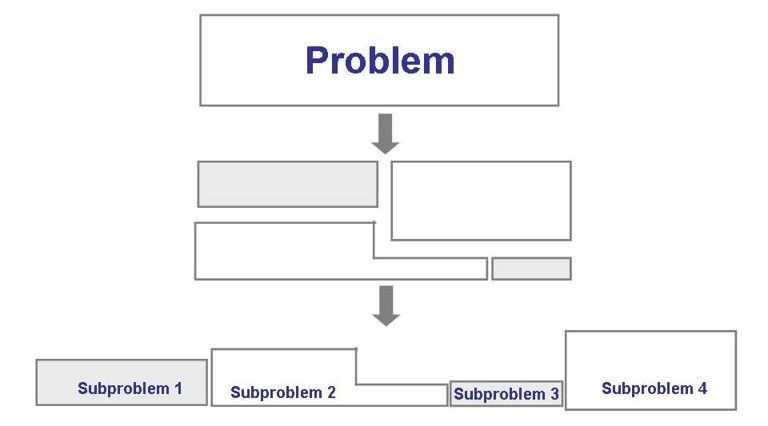
\includegraphics[width=\textwidth]{analysis}
    \item Sintetico: Costruisco dai sotto-problemi la soluzione al problema di partenza
    
    L'integrazione dei sotto-problemi è difficile
    
    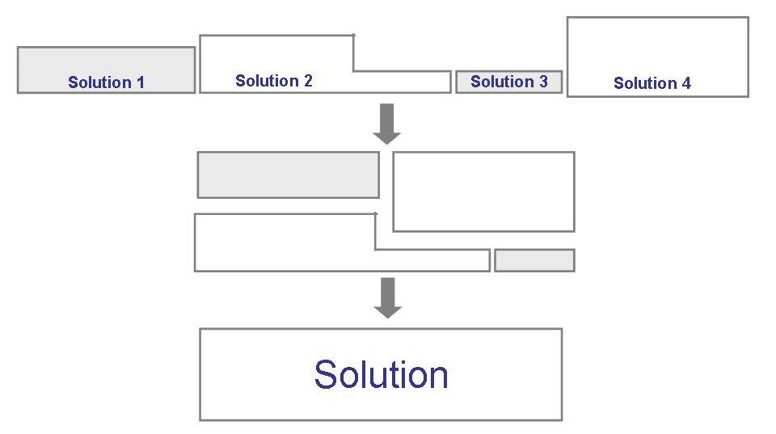
\includegraphics[width=\textwidth]{synthesis.jpg}
\end{itemize}

\subsection{Processo SW; MODELLO dei Processi SW; modelli generici}
\begin{itemize}
    \item Processo Software: Un insieme di attività correlate il cui obiettivo è lo sviluppo o l'evoluzione del software
    \item Modello dei processi: Una rappresentazione semplificata di un processo software, presentata da una prospettiva specifica
    \item Modelli generici: Waterfall, Evolutionary development, Formal transformation, Integration from reusable components, \dots 
\end{itemize}

\subsection{Parametri di Qualità del SW: manutenibilità, ‘potersi fidare’, sicurezza \& protezione, efficienza, accettabilità}
\begin{itemize}
    \item Manutenibilità: Il software deve poter evolversi facilmente per soddisfare le mutevoli esigenze
    \item Affidabilità e sicurezza: Il software deve essere affidabile, sicuro (Protezione: non danneggiare i propri dati) e protetto (Sicurezza: non provocare danni a cose, persone, \dots)
    \item Efficienza: Il software non dovrebbe fare uno spreco di risorse di sistema (non è più un problema così importante come in passato)
    \item Accettabilità: Il software deve essere accettabile per il tipo di utenti per cui è progettato. Ciò significa che deve essere comprensibile, utilizzabile e compatibile con altri sistemi che usano
\end{itemize}

\subsection{Le grandi sfide attuali dell’IS: sistemi Legacy, eterogeneità hd e SW, richiesta di velocità nello sviluppo e nella delivery}
\begin{itemize}
    \item Legacy system: sistemi vecchi e preziosi devono essere mantenuti e aggiornati
    \item Eterogeneità: sempre più spesso i sistemi devono funzionare come sistemi distribuiti su reti che includono diversi tipi di computer e dispositivi mobili
    \item Consegna, sicurezza e fiducia: i cambiamenti aziendali, sociali e culturali stanno causando una crescente pressione per una consegna più rapida del software
\end{itemize}

\subsection{Web e IS}
\begin{itemize}
    \item Il Web è ora una piattaforma per l'esecuzione di applicazioni e organizzazioni stanno sviluppando sempre più sistemi basati sul Web piuttosto che sistemi locali.
    \item I servizi Web consentono l'accesso alle funzionalità dell'applicazione sul Web.
    \item Il cloud computing è un approccio alla fornitura di servizi informatici in cui le applicazioni vengono eseguite in remoto sul "cloud".
    \item Gli utenti non acquistano software ma pagano in base all'uso (SaS - Software ad a Service).
    \item Il riutilizzo del software è l'approccio dominante per la costruzione di sistemi basati sul Web.
    \item I sistemi basati sul Web dovrebbero essere sviluppati e distribuiti in modo incrementale.
    \item Le interfacce utente sono vincolate dalle capacità dei browser Web.
\end{itemize}
\newpage

\section{Ingegneria dei sistemi hardware software}
\subsection{Concetto generale di Sistema. I sistemi che ci interessano includono HW SW e aspetti organizzativi (persone, processi).}
\begin{itemize}
    \item Una raccolta mirata di componenti interconnessi che lavorano insieme verso un obiettivo comune. Un sistema può includere software, hardware meccanico, elettrico ed elettronico ed essere gestito da persone. I componenti di sistema dipendono da altri componenti di sistema. Le proprietà e il comportamento dei componenti del sistema sono indissolubilmente mescolati
\end{itemize}
\subsection{Problematiche dell’ingegneria dei sistemi e relazioni con l’IS.}
\begin{itemize}
    \item I sistemi di grandi dimensioni sono generalmente progettati per risolvere problemi "malvagi"
    \item L'ingegneria dei sistemi richiede un grande coordinamento in tutte le discipline
    \begin{itemize}
        \item Quasi infinite possibilità di compromessi di progettazione tra i componenti
        \item Diffidenza reciproca e mancanza di comprensione tra le discipline ingegneristiche
    \end{itemize}
    \item I sistemi devono essere progettati per durare molti anni in un ambiente che cambia
    \item La percentuale di software nei sistemi è in aumento. L'elettronica per uso generale basata su software sta sostituendo i sistemi per uso speciale
    \item I problemi di ingegneria dei sistemi sono simili ai problemi di ingegneria del software
    \item Il software è (purtroppo) visto come un problema nell'ingegneria dei sistemi. Molti grandi progetti di sistema sono stati ritardati a causa di problemi del software
    \item Spesso viene richiesto al software di "compensare" la "rigidità" dell'hardware!
    \item E’ quindi necessario inquadrare l’attività di sviluppo del SW nel ambito più vasto e generale del processo di ingegnerizzazione del Sistema in cui il SW sarà inserito.
    \item Bisogna quindi considerare lo scopo del Sistema, i requisiti (di business) cui va incontro, i ruoli delle varie componenti (varie tipologie di dispositivi HW, le persone e i processi coinvolti, alter procedure a DB coinvolti, …)
    \item Concentrarsi solo e immediatamente sul SW senza avere una visione più generale ‘di Sistema’ non è corretto!
\end{itemize}
\subsection{Proprietà emergenti. P. funzionale e p. non funzionali. Shall-not properties.}
\begin{itemize}
    \item Proprietà emergenti: sono proprietà del sistema visto come tutt'uno piuttosto che proprietà dei singoli componenti e sono conseguenze delle relazioni tra i componenti del sistema (possono essere misurate solo dopo l'integrazione dei vari componenti nel sistema). Es. peso, usabilità e affidabilità.
    \item Proprietà (emergenti) funzionali: riguardano \textbf{come un sistema funziona}, i.e. la relazione input/ouput. Es. una bicicletta ha la proprietà funzionale di essere un dispositivo di trasporto una volta assemblata dai suoi componenti.
    \item Proprietà (emergenti) non funzionali: riguardano il \textbf{comportamento del sistema} nel suo ambiente operativo. Es. affidabilità, prestazioni, sicurezza, usabilità e protezione.
    \item \textit{shall-not properties}: sono proprietà che il sistema \textbf{non dovrebbe esibire}.
\end{itemize}
\subsection{Cambiamento dei fattori umani/organizzativi e loro importanza.}
\begin{itemize}
    \item Process changes: Il sistema richiede modifiche ai processi di lavoro nell'ambiente?
    \item Job changes: Il sistema diminuisce le abilità degli utenti in un ambiente o fa cambiare il loro modo di lavorare?
    \item Organisational changes: Il sistema cambia la struttura del potere politico in un'organizzazione?
\end{itemize}
\subsection{Processo di systems engineering e fasi principali.}
\begin{itemize}
    \item in genere si usa il modello \textit{waterfall} che consiste nella definizione dei requisiti, nel design del sistema, nello sviluppo dei sottosistemi, nell'integrazione, poi l'installazione, l'evoluzione e infine la de-commissione.
\end{itemize}
\subsection{Problemi nel System requirements}
\begin{itemize}
     \item Modifica in base al sistema specificato
     \item È necessario anticipare gli sviluppi hardware/comunicazioni per tutta la durata del sistema
     \item Difficile definire requisiti non funzionali (in particolare) senza un'impressione della struttura dei componenti del sistema.
\end{itemize}
\subsection{Problemi nel System design}
\begin{itemize}
     \item I requisiti di partizionamento su hardware, software e componenti umani possono comportare molte negoziazioni
     \item Spesso si presume che i problemi di progettazione difficili vengano risolti prontamente utilizzando il software
     \item Le piattaforme hardware potrebbero non essere appropriate per i requisiti software, quindi il software deve compensare questo
\end{itemize}
\subsection{Evoluzione e legacy}
\begin{itemize}
    \item I grandi sistemi hanno grandi periodi di vita, devono evolvere per rispettare i requisiti in cambiamento.
    \item Sistemi legacy: sistemi ancora in uso che sono stati sviluppati nel passato con tecnologie, metodologie, procedure, lavorazioni \dots che sono nel frattempo diventate obsolete, ciò li rende di difficile cambiamento perché la modifica di un componente comporta la modifica di altri componenti.
\end{itemize}
\subsection{System Procurement: due possibilità, modello dei processi}
\begin{itemize}
    \item sviluppo del sistema da parti pre-confenzionate (COTS -- components off the shelf)
    \item sviluppo del sistemi da zero (esempio hardware: si scelgono i vari componenti: cpu, bluetooth, memoria, porte \dots e vengono montate su una board)
\end{itemize}
\subsection{Modello Contractor/subcontractor}
\begin{itemize}
    \item La fornitura di grandi sistemi hardware/software si basa generalmente su alcuni principali contraenti
    \item I sotto-contratti vengono stipulati con altri fornitori per alcune parti del sistema
    \item Il cliente è in contatto con il contraente principale e non tratta direttamente con i sotto-contraenti
    
    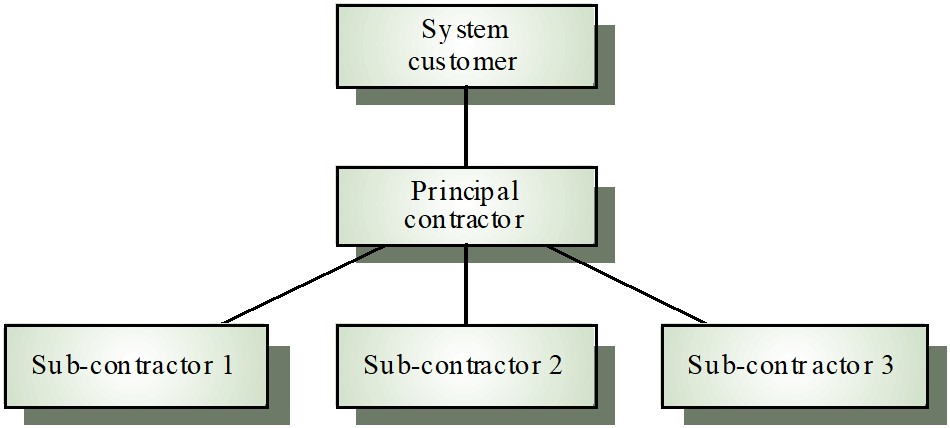
\includegraphics[width=\textwidth]{Contractor-subcontractor.jpg}
\end{itemize}
\newpage

\section{Processi software}
\subsection{Processo, processo sw, modello di processo, elementi caratteristici dei processi}
\begin{itemize}
    \item Processo:Un insieme coerente di attività per specificazione, progettazione, implementazione e testing di sistemi software.
    \item processo software: Un insieme strutturato di attività necessarie per sviluppare un sistema software
    \item modello di processo software: è una rappresentazione astratta di un processo che presenta una descrizione da una prospettiva particolare.
    \item Elementi caratteristici dei processi:
    \begin{description}
        \item[Input] ciò che il processo considera come punto di partenza, da trasformare nei risultati dell'esecuzione del processo
        \item[Prodotti o output] quali sono i risultati di un'attività di processo
        \item[Ruoli] che riflettono le responsabilità delle persone coinvolte nel processo
        \item[Risorse] necessario per l'esecuzione del processo
        \item[Pre/Post condizione] che sono affermazioni vere prima e dopo l'attivazione di un'attività di processo o la produzione di un prodotto.
    \end{description}
\end{itemize}
\subsection{Processi plan-driven, processi agili}
\begin{itemize}
    \item \textit{plan-driven}: sono processi dove tutti i processi sono pianificati \textbf{in anticipo} e il progresso è misurato rispetto al piano.
    \item Nei processi agili, la pianificazione è incrementale ed è più semplice modificare il processo per riflettere le mutevoli esigenze dei clienti.
    \item in pratica, la maggior parte dei processi pratici include elementi sia dai \textit{plan-driven} che dagli approcci agili.
\end{itemize}
\subsection{Waterfall Model, caratteristiche, pregi, criticità}
\begin{itemize}
    \item In un modello a cascata, ogni fase deve essere completata prima che possa iniziare la fase successiva e non vi sono sovrapposizioni nelle fasi che sono:
    \begin{itemize}
        \item definizione dei requisiti
        \item system design
        \item implementazione e unit testing
        \item integrazione e testing del sistema
        \item \textit{deployment}
        \item oparatività e manutenzione
    \end{itemize}
    \item Pregi: gode di una buona visibilità e gestibilità dovuta al fatto che nel passaggio da una fase alla successiva corrisponde la stesura di un documento (analisi dei requisiti, di progetto, di sorgenti, di rapporto tecnico\dots) consegnato e accettato dal committente.
    \item Criticità: La suddivisione non flessibile del progetto in fasi distinte rende difficile rispondere alle mutevoli esigenze dei clienti
\end{itemize}
\subsection{Prototyping/evolutionary development: exploratory prototyping, throw-away prototyping; ciclo iterativo del prototyping; vantaggi, criticità e applicabilità}
\begin{itemize}
    \item \textit{prototyping} si costruiscono e si valuta diverse versioni successive del sistema, al fine di avere più informazioni ed idee sul risultato finale che si vuole ottenere e sul come ottenerlo. Il Sistema può essere di ‘dimensione reali’ o ‘in scala ridotta’.
    \item l'\textit{evolutionary development} si divide in:
    \begin{description}
        \item[exploratory development/prototyping] l'obiettivo è lavorare con i clienti e far evolvere un sistema finale da una specifica di struttura iniziale. Dovrebbe iniziare con requisiti ben compresi, iniziando con ciò che è chiaro e cercando di capire il resto.
        \item[throw-away prototyping] L'obiettivo è comprendere i requisiti di sistema. Dovrebbe iniziare con requisiti poco compresi. Un prototipo viene sviluppato "veloce e sporco", quindi, quando i requisiti sono stati compresi, il prototipo viene gettato via. Concentrando solo su ciò che non è chiaro, al fine di capirlo meglio.
    \end{description}
    \item il modello \textit{evolutionary} è suddiviso nelle seguenti fasi:
    \begin{itemize}
        \item specifica
        \item sviluppo (che produce un prototipo)
        \item validazione
    \end{itemize}
    che possono essere ripetuti più volte, fino al completamento del sistema.
    \item vantaggi:
    \begin{itemize}
        \item riduzione dei costi implementativi se i requisiti cambiano
        \item più feedback dal client
    \end{itemize}
    \item criticità
    \begin{itemize}
        \item mancanza di visibilità
        \item sistemi spesso mal strutturati
        \item possono essere richieste abilità particolari (e.g. in linguaggi per la rapida prototipizzazione)
    \end{itemize}
    \item applicabilità
    \begin{itemize}
        \item per piccoli/medi sistemi interattivi
        \item per tecnologie e sistemi innovativi
        \item per parti di un grande sistema (e.g. user interface)
        \item per sistemi con una breve durata di vita
    \end{itemize}
\end{itemize}
\subsection{Modelli IBRIDI}
Sono modelli che integrano più aspetti insieme.  Ad esempio, il modello waterfall integrato con il prototyping è un waterfall dove allo stadio del sistem testing è possibile tornare indietro all'analisi dei requisiti o al design del sistema.
\subsection{Formal system development: l’idea e i suoi limiti}
È una metodologia che si basa su una serie di trasformazioni di una specifica espressa in linguaggio matematico per giungere a un programma eseguibile.  Si tratta di un processo incrementale che a ogni step viene provato essere corretto.  Si tratta di un modello di scarso utilizzo pratico.
\subsection{Sviluppo basato sul ri-uso: strutturazione in fasi}
Basato sull'idea del riuso sistematico dove il sistema viene integrato da componenti esistenti o COTS (\textit{commercial off-the-shelf}).

Fasi del processo:
\begin{enumerate}
    \item Analisi dei componenti
    \item Modifica dei requisiti
    \item Progettazione del sistema con riutilizzo
    \item Sviluppo e integrazione
\end{enumerate}

\subsection{Cicli di Processo, iterazione; sviluppo incrementale, incrementi, vantaggi e criticità; sviluppo iterativo}
\begin{itemize}
    \item I requisiti di sistema sono \textbf{sempre in cambiamento} nel corso di un progetto.

    Ci sono due approcci collegati:
    \begin{itemize}
        \item Sviluppo incrementale, e la sua variante denominata Sviluppo iterativo
        \item Sviluppo a spirale
    \end{itemize}
    
    \item Sviluppo incrementale:
    \begin{itemize}
        \item Combina il Waterfall con il modello evolutivo
        \item Lo sviluppo e il rilascio è diviso in \textbf{incrementi} ognuno con una parte delle funzionalità richieste
        \item I requisiti utente sono prioritari e i requisiti di massima priorità sono inclusi nei primi incrementi
        \item Una volta avviato lo sviluppo di un incremento, i requisiti vengono congelati sebbene i requisiti e gli incrementi successivi possano continuare ad evolversi
    \end{itemize}
    
    \item vantaggi:
    \begin{itemize}
        \item Le funzionalità vengono consegnate incrementalmente con ogni rilascio quindi le funzionalità sono disponibili prima: non si deve attendere il completamento di tutto il sistema.
        \item I primi incrementi fungono da prototipi per aiutare la raccolta dei requisiti per i successivi incrementi
        \item Minor rischio di fallimento generale del progetto
        \item I primi incrementi(che hanno la priorità più alta) sono quelli più testati e più sicuri
    \end{itemize}
    
    \item svantaggi:
    \begin{itemize}
        \item Non avendo specifiche complete all'inizio risulta difficile trovare i \enquote{giusti} incrementi per scomporre il sistema
        \item Difficile identificare servizi comuni (strutture di base)
        \item Può richiedere modelli contrattuali non standard o più contratti successivi
    \end{itemize}
    
    \item Sviluppo iterativo: inizia con il sistema completo, quindi cambia funzionalità/implementazione di ciascun sottosistema con ogni nuova versione
\end{itemize}

\subsection{Extreme programming}
\begin{itemize}
    \item Nuovo approccio allo sviluppo basato sullo sviluppo e sulla fornitura di incrementi di funzionalità molto piccoli
    \item Si affida al costante miglioramento del codice, al coinvolgimento degli utenti nel team di sviluppo e alla programmazione a coppie
\end{itemize}
\subsection{Rischio: definizione e ruolo; cause di fallimento di un progetto sw; Modello di sviluppo a spirale, settori della spirale}
Le cause per le quali un progetto di sviluppo software
\begin{itemize}
    \item Requisiti incompleti o vaghi, conflitti tra gli \textit{stakeholders}
    \item Mancanza di coinvolgimento degli utenti
    \item Mancanza di risorse, skill non sufficienti per il lavoro
    \item Aspettative non realistiche
    \item Cattiva gestione del progetto, pianificazione o stima dei costi
    \item Scarso supporto esecutivo
    \item Mancanza di comunicazione
    \item Modifica dei requisiti e delle specifiche
    \item Scarsa architettura
    \item Rilevamento di segnali di avviso di guasto ritardato
\end{itemize}

Il modello a spirale:
\begin{itemize}
    \item Il processo è rappresentato come una spirale piuttosto che come una sequenza di attività con backtracking
    \item Ogni ciclo nella spirale rappresenta una fase del processo.
    \item Nessuna fase fissa come specifica o design - i loop nella spirale sono scelti a seconda di ciò che è richiesto
    \item I rischi vengono esplicitamente valutati e risolti durante l'intero processo
    \item Si parte dalle attività che hanno il più alto livello di rischio.
\end{itemize}
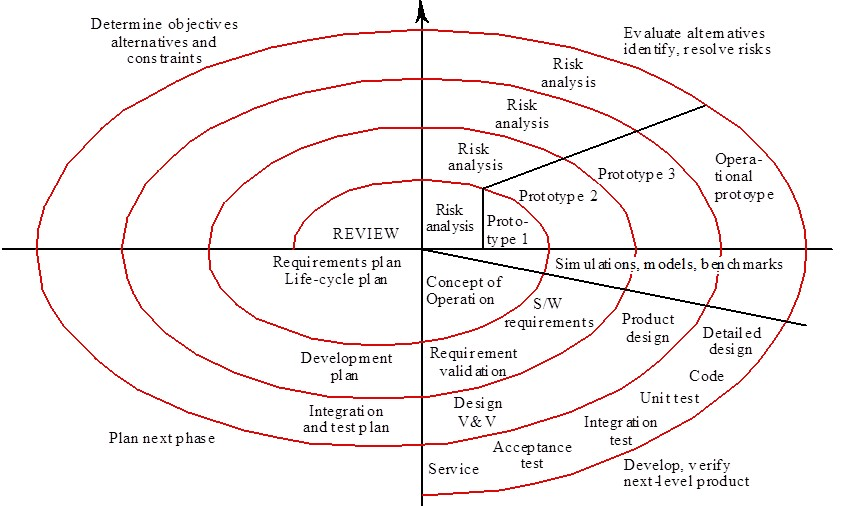
\includegraphics[width=\textwidth]{spirale.jpg}

Settori della spirale:
\begin{itemize}
    \item Definizione degli obiettivi: vengono identificati obiettivi specifici per la fase
    \item Valutazione e riduzione del rischio: vengono valutati i rischi e vengono messe in atto attività per ridurre i rischi chiave
    \item Sviluppo e validazione: viene scelto un modello di sviluppo per il sistema che può essere uno qualsiasi dei modelli generici
    \item Pianificazione: il progetto viene rivisto e viene pianificata la fase successiva della spirale
\end{itemize}
\subsection{Attività fondamentali dei processi primari per lo sviluppo del sw}
\begin{description}
    \item[\red{Analisi dei requisiti} e \blue{specifiche sw}] \red{Il processo di analisi delle esigenze} e \blue{di determinazione dei servizi richiesti e dei vincoli} per il funzionamento e lo sviluppo del sistema. Studio di fattibilità, Richiamo e analisi dei requisiti, Specifica dei requisiti e Convalida dei requisiti
    \item[Progettazione e realizzazione] Il processo di conversione delle specifiche di sistema in un sistema eseguibile. Le attività di progettazione e realizzazione sono strettamente correlate e possono essere interrelate.
    \item[Validazione] \red{La verifica} e \blue{la convalida} hanno lo scopo di dimostrare che un sistema \red{è conforme alle sue specifiche} e \blue{soddisfa realmente le esigenze e i requisiti del cliente del sistema}
    \item[Evoluzione] Il software è intrinsecamente flessibile e può cambiare. Poiché i requisiti cambiano in base alle mutevoli circostanze aziendali, anche il software che supporta l'azienda deve evolversi e cambiare. Sebbene ci sia stata una delimitazione tra sviluppo ed evoluzione (manutenzione), ciò è sempre più irrilevante in quanto sempre meno sistemi sono completamente nuovi
\end{description}
\subsection{Definizione di CASE, varietà delle funzionalità e copertura dell’intero ciclo di vita}
\begin{description}
    \item[CASE] Computer-aided software engineering è un software a supporto dello sviluppo del software e dei processi di evoluzione
\end{description}
\newpage

\addtocounter{section}{-1}
\section{Modelli processi ISO}
\subsection{Processi sw primari, di supporto e di gestione; loro relazioni}
\begin{description}
    \item[Processi primari] attività necessarie a specificare, progettare, produrre, mantenere ed estendere il prodotto SW
    \item[Processi di supporto] vengono eseguiti parallelamente ai processi primari al fine di supportarli e garantire la qualità ed il successo del progetto 
    \item[Processi di gestione] attività necessarie a gestire il progetto di sviluppo del prodotto SW
\end{description}
\subsection{Ciclo di Vita, definizione, caratteristiche, organizzazione}
\begin{itemize}
    \item Il Ciclo di Vita specifica come sono definiti e organizzati i vari task coinvolti nella progettazione, costruzione e manutenzione di un prodotto (artifact). Più precisamente è uno schema di riferimento che specifica in modo astratto e generale quali task svolgere e quando svolgerli.
    \item Il livello di definizione del ciclo di vita si presenta:
        \begin{itemize}
            \item astratto, poiché prescinde da dettagli tecnico/implementativi
            \item generale, poiché solitamente ricomprende una vasta gamma di casistiche ed è indipendente da contesti specifici
        \end{itemize}
    \item Organizzazione: il ciclo di vita è basato su una struttura a due livelli: il livello delle fasi con i passi principali e il livello dei task con i compiti da svolgere per ogni fase. Le fasi sono raggruppate in macrofasi e i task sono raggruppati in step
\end{itemize}
\subsection{Metodologia di sviluppo, definizione e caratteristiche}
\begin{description}
    \item[Metodologia di sviluppo] è un insieme integrato di metodi con i quali eseguire effettivamente tutti i singoli task del ciclo di vita.
    \item[Livello di definizione] di una metodologia di sviluppo si presenta:
    \begin{description}
        \item[Concreto], poiché riguarda tutti i dettagli tecnico/implementativi
        \item[Specifico] poiché solitamente tiene conto dello specifico contesto in cui è definita la metodologia
    \end{description}
\end{description}
\subsection{Metodi tecnici e metodi di gestione}
Un metodo è un insieme integrato di:
\begin{itemize}
    \item tecniche
    \item procedure
    \item linguaggi, notazioni
    \item strumenti
    \item standard, formati
    \item documentazione
    \item best practice
    \item criteri, linee guida, vincoli
\end{itemize}
\newpage

\end{document}
